\section{Towards stable software artifacts} \label{sec:on_stability}

\gls{ns} originated in the field of software engineering, aiming to achieve modular and
stable software artifacts. However, the underlying theory of \gls{ns} can be applied to
various other domains, such as Enterprise Engineering, Business Process Modeling, and
document management. This research acknowledges the software engineering background of
gls{ns}. It consistently refers to software and Information Systems when referring to
\enquote*{artifacts}. However, the reader should realize that the concepts and artifacts
are not restricted to software artifacts alone.

In many scientific disciplines, stability is defined as \emph{Bounded Input Bounded
Output} (BIBO). It is the fundamental property of a system when subjected to bounded input
disturbances. BIBO stability ensures that the output of a system will also be bounded,
preventing uncontrolled or unexpected behavior \parencite[270]{mannaert_normalized_2016}. 

A real-world example of the importance of stability is the Tacoma Narrows Bridge in
Washington State, USA. The bridge, depicted in figure \ref*{fig:bridge}, collapsed on
November 7, 1940, due to wind-induced oscillations called aeroelastic flutter. The wind (Input)
induced oscillations in the bridge, causing it to start swaying back and forth (Output). These
oscillations were initially small, but as they continued, they began to increase in
amplitude or magnitude, causing the bridge to collapse.

\begin{figure}[H]
    \centering
    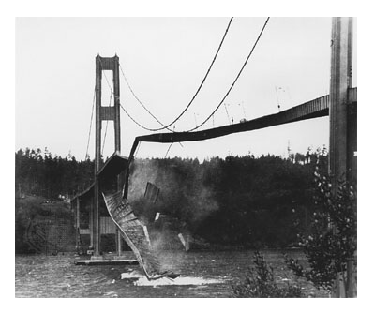
\includegraphics[width=0.6\textwidth]{Figures/bridge.pdf}
    \caption[TNB]{Tacoma Narrows Bridge (Galloping Gertie)}
    \label{fig:bridge}
\end{figure}

In the context of NS stability can be translated to software artifacts also. It is
considered a critical property, ensuring that the software is not excessively sensitive to
small changes \autocite[270]{mannaert_normalized_2016}. New functional requirements should
only lead to fixed, and an expected amount of changes in the source code. Conversely,
instabilities occur when the total number of modifications relies on the size of the
software artifact. The number of changes will grow over time in parallel with the growth
of the software artifact. These instabilities are referred to as combinatorial effects
\autocite[270]{mannaert_normalized_2016}. when combinatorial effects are absent, the
software artifact can be considered evolvable.